\documentclass{article}
\usepackage{amsmath,amssymb}
\usepackage{tikz}
\usetikzlibrary{arrows.meta,positioning,calc,shapes.geometric}
\pagestyle{empty}
\begin{document}
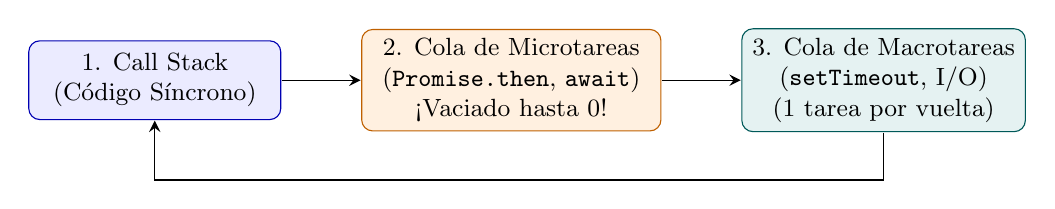
\begin{tikzpicture}
\tikzset{node distance=1.6cm, >=stealth, thick, font=\small}
\node[draw=blue!70!black, fill=blue!8, rounded corners, minimum width=3.2cm, minimum height=1.0cm, align=center] (stack) {1. Call Stack\\(Código Síncrono)};
\node[draw=orange!75!black, fill=orange!12, rounded corners, minimum width=3.8cm, minimum height=1.0cm, align=center, right=1.0cm of stack] (micro) {2. Cola de Microtareas\\(\texttt{Promise.then}, \texttt{await})\\¡Vaciado hasta 0!};
\node[draw=teal!70!black, fill=teal!10, rounded corners, minimum width=3.6cm, minimum height=1.0cm, align=center, right=1.0cm of micro] (macro) {3. Cola de Macrotareas\\(\texttt{setTimeout}, I/O)\\(1 tarea por vuelta)};
\draw[->] (stack) -- (micro);
\draw[->] (micro) -- (macro);
\draw[->] (macro.south) -- ++(0,-0.6) -| (stack.south);
\end{tikzpicture}
\end{document}
